% !TeX root = ../defense.tex

\section{Results}
\frame{\sectionpage}

\begin{frame}{Entropy measures}
\centering
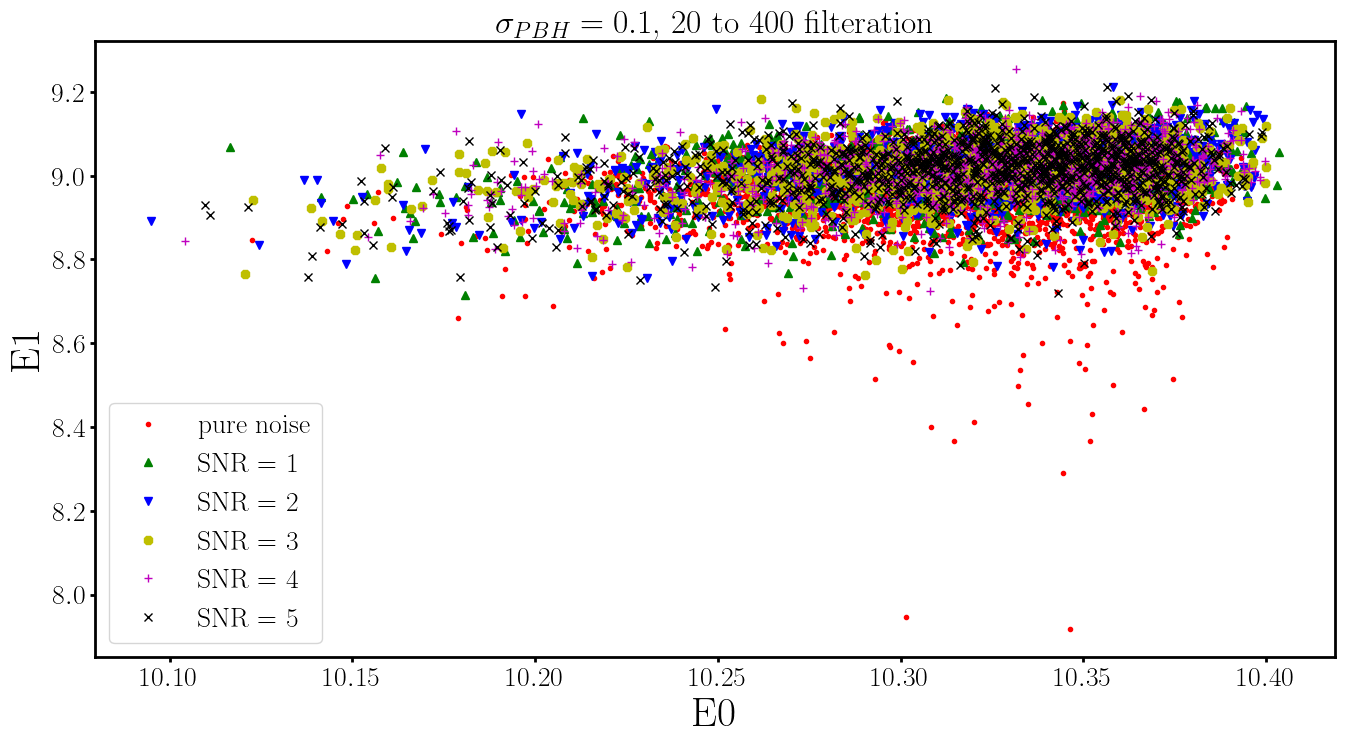
\includegraphics[height=.8\textheight]{img/E0_E1_SNR}
\end{frame}

\begin{frame}{Distance measures}
	\centering
	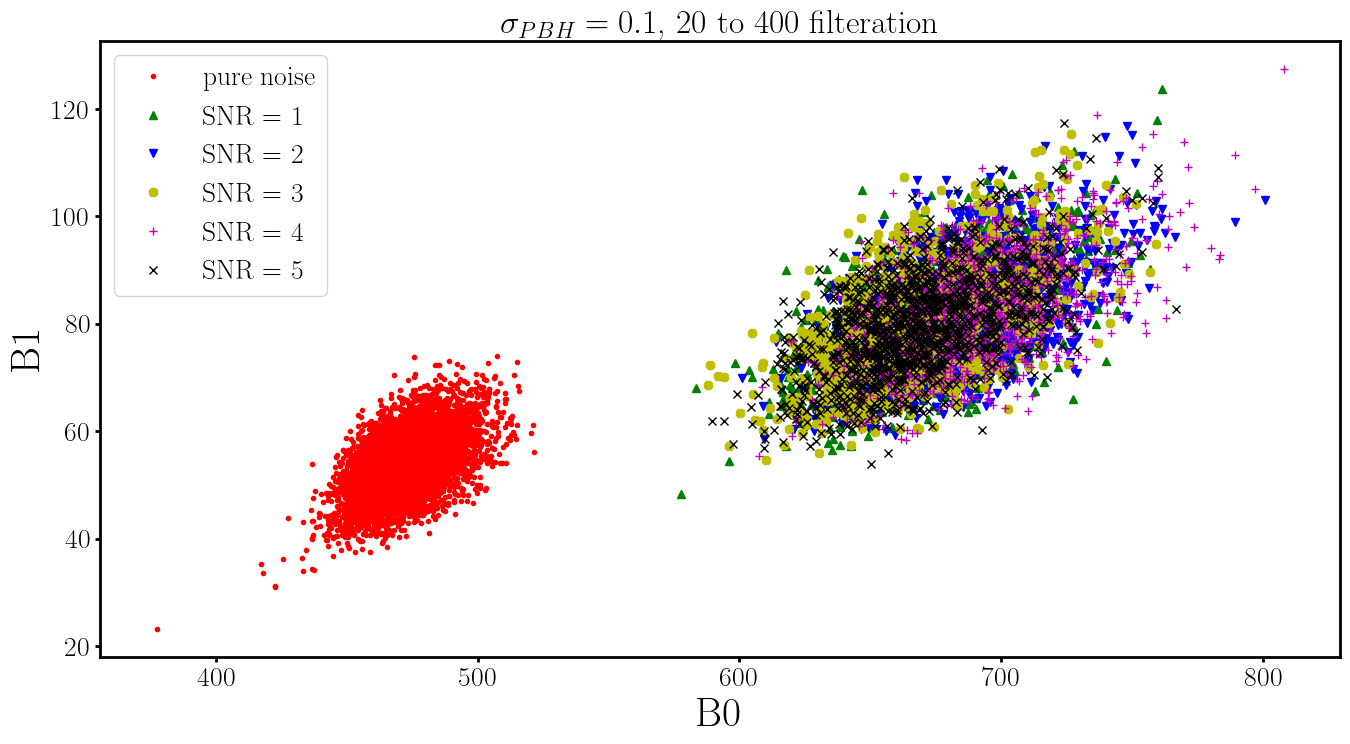
\includegraphics[height=.8\textheight]{img/B0_B1_SNR}
\end{frame}

\begin{frame}{Distance measures}
	\centering
	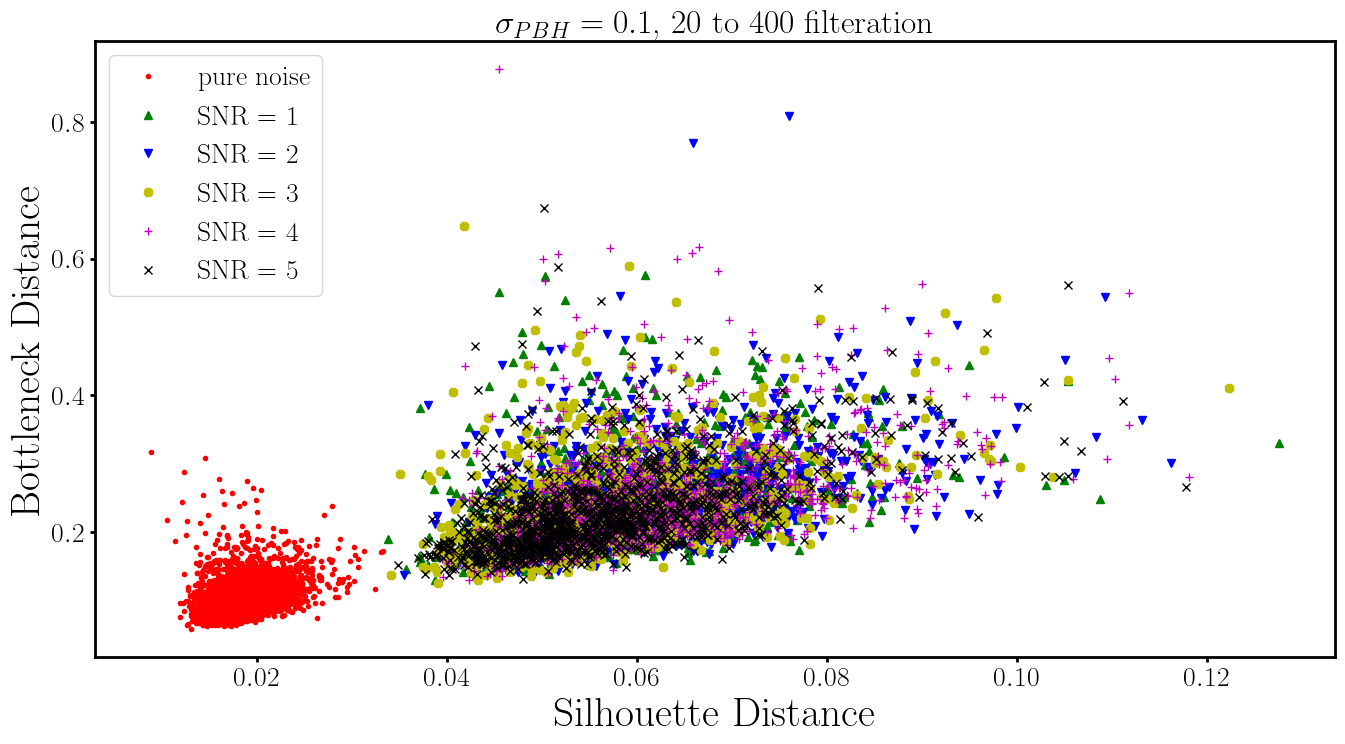
\includegraphics[height=.8\textheight]{img/SD_BD_SNR}
\end{frame}

\begin{frame}{Image measures}
	\centering
	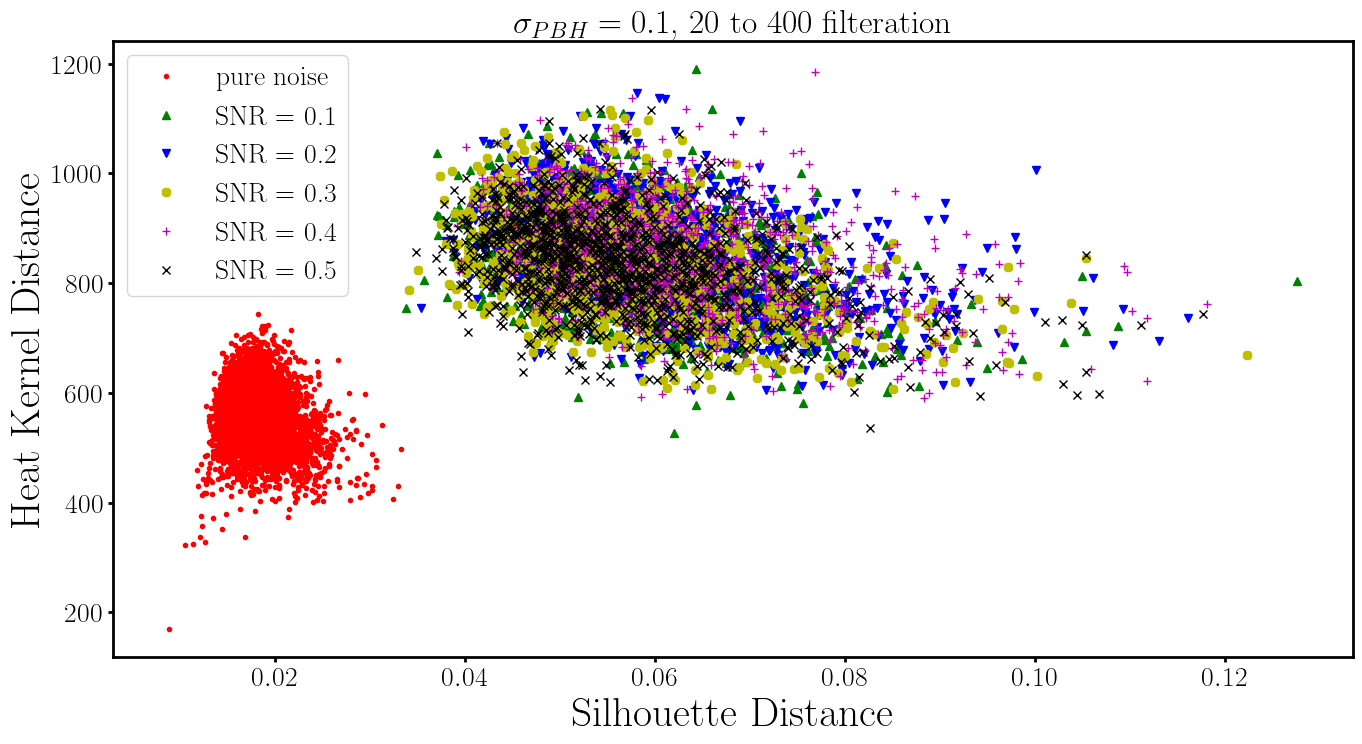
\includegraphics[height=.8\textheight]{img/SD_HK_SNR}
\end{frame}

\begin{frame}{First attempt to classification}
	\centering
	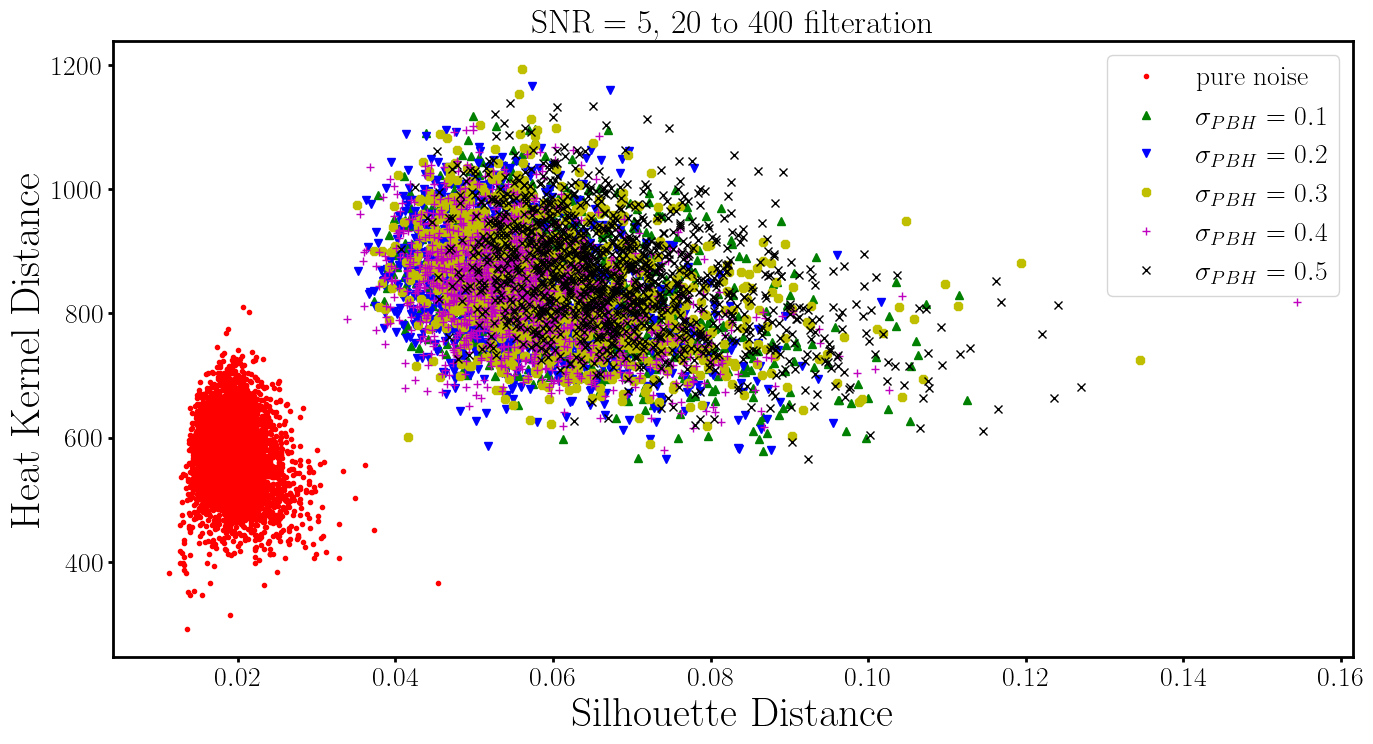
\includegraphics[height=.8\textheight]{img/SD_HK_sig}

\end{frame}

\begin{frame}{What did we learn?}
\begin{enumerate}[<+->]
	\item In contrast to the result from \href{https://arxiv.org/abs/1910.08245}{Bresten and Jung}, entropy measures are not good for detecting a stochastic background.\\~\\
	\item Betti, Silhoutte and Heat Kernel amplitudes when combined together two by two, are very resiliant to noise.\\~\\
	\item The best topological measure to use for detecting the presence of a signal is Betti distance beacuse it's simpler to calculate.\\~\\
	\item Scaler topological measures can not classify the signals based on their physical parameters.\\~\\
\end{enumerate}
\uncover<+->{Hence to build a classification pipeline, we need to use more complicated topological measures.}
\end{frame}

\begin{frame}{A classification pipeline}
	\centering
	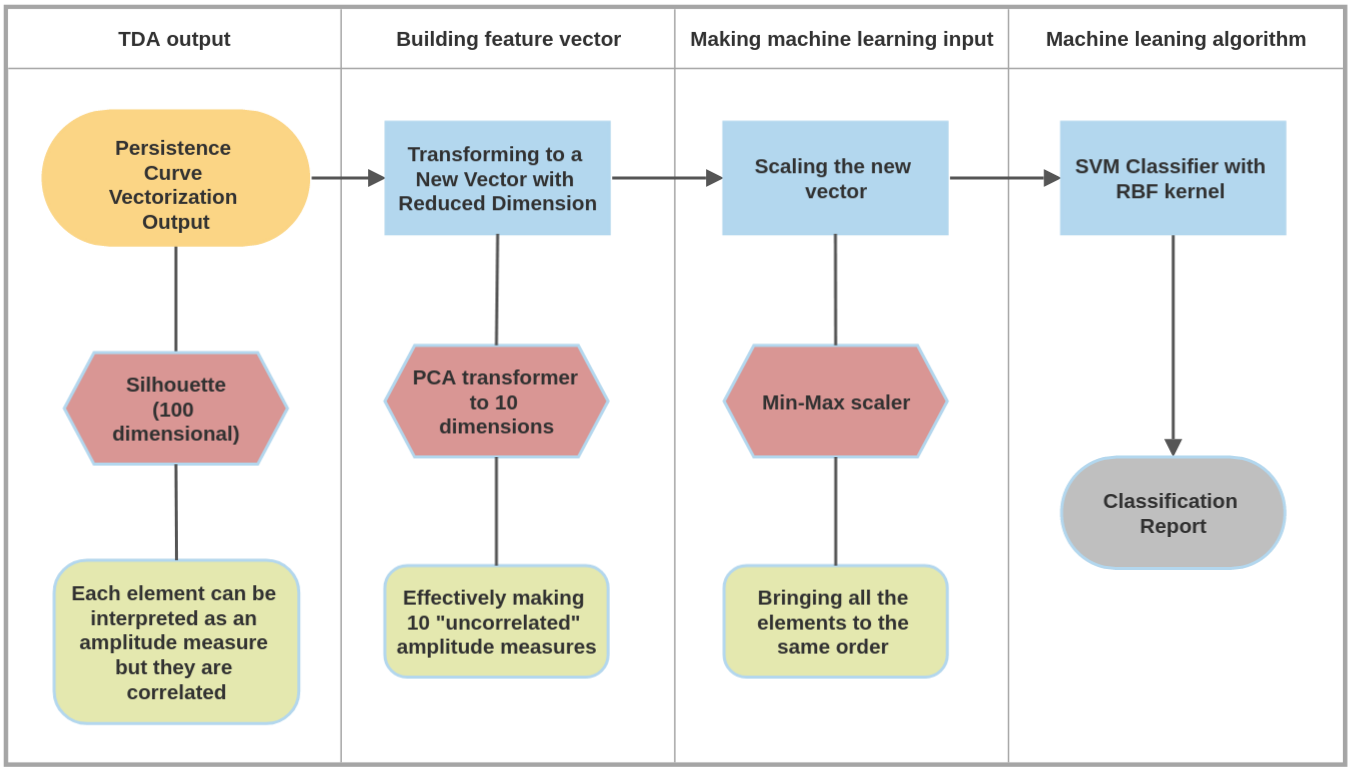
\includegraphics[height=.8\textheight]{img/Classification_algorithm}
\end{frame}

\begin{frame}{Classification report}
\vskip .5cm
\centering
\begin{tabular}{lcccc}
	\textbf{Physical parameter} & \textbf{precision (\%)} & \textbf{recall (\%)} & \textbf{f1-score} & \textbf{support} \\
	\hline \hline
	$\sigma_{PBH}$ = 0.10 & 91 & 85 & 0.88 & 379 \\
	$\sigma_{PBH}$ = 0.15 & 81 & 86 & 0.83 & 345 \\
	$\sigma_{PBH}$ = 0.20 & 93 & 93 & 0.93 & 357 \\
	$\sigma_{PBH}$ = 0.25 & 88 & 94 & 0.91 & 375 \\
	$\sigma_{PBH}$ = 0.30 & 85 & 93 & 0.89 & 328 \\
	$\sigma_{PBH}$ = 0.35 & 95 & 91 & 0.93 & 373 \\
	$\sigma_{PBH}$ = 0.40 & 99 & 97 & 0.98 & 347 \\
	$\sigma_{PBH}$ = 0.45 & 94 & 81 & 0.87 & 366 \\
	$\sigma_{PBH}$ = 0.50 & 89 & 93 & 0.91 & 367 \\
	$\sigma_{PBH}$ = 0.55 & 85 & 87 & 0.86 & 367 \\
	\hline 
	accuracy        &    &    & 0.9 & 3604 \\
	macro avrage    & 90 & 90 & 0.9 & 3604 \\
	\hline \hline
\end{tabular}
\vskip.3cm
\begin{align*}
\uncover<2->{
	\mathrm{precision} = \frac{\mathrm{TP}}{\mathrm{TP} + \mathrm{FP}},\qquad
}
\uncover<3->{
	\mathrm{recall} = \frac{\mathrm{TP}}{\mathrm{TP} + \mathrm{FN}},\qquad
}
\uncover<4->{
	\mathrm{f1-score} = 2 \frac{\mathrm{recall} \times \mathrm{precision}}{\mathrm{recall} + \mathrm{precision}}
}
\end{align*}
\end{frame}